\subsection{Front Panel}

The front panel of the acquisiton module has the 20-pin input for all
8 differential channel pairs of amplifier input.

The pinout can be seen in figure \ref{inputconn}. 


\begin{figure}[h!]
\centering
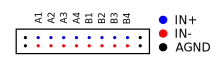
\includegraphics[scale=1.0]{enclosure.front.inputconn.svg}
\caption{The front panel connector for the Soma Acquisition Module.
  AGND is connected to the amplifier analog ground.  }
\label{inputconn}
\end{figure}

The connector is a dual-row, twenty-pin 0.100-inch pitch IDC
connector.


\subsection{Back Panel}
The back panel (Figure \ref{backpanel}) contains power, IO, and
debugging information. There are four sections of interest.

\begin{figure}[h!]
\centering
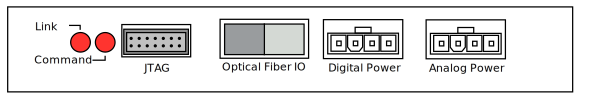
\includegraphics[scale=1.0]{enclosure.back.svg}
\caption{The back of the Soma Acquisition Module.}
\label{backpanel}
\end{figure}

\subsubsection{Status LEDs}
There are two status LEDs on the back of the module:
\begin{itemize}
\item \textbf{Link} : indicates the link with the Soma backplane (over the optical fiber)
is functioning properly. 
\item \textbf{Command}: Flashes briefly every time the Soma Backplane sends a command to the 
acqboard. 
\end{itemize}

\subsubsection{JTAG port}
The JTAG port (figure \ref{jtag}) is the standard 14-pin 2mm-pitch JTAG connector for
Xilinx FPGAs, allowing both programming of the on-board flash and
debugging.

\begin{figure}[h!]
\centering
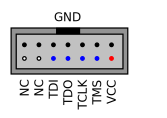
\includegraphics[scale=1.0]{enclosure.back.jtag.svg}
\caption{The JTAG port.}
\label{jtag}
\end{figure}

\subsubsection{Optical Fiber IO}
The optical fiber interface (figure \ref{fiber}) takes two 1-mm
visible-light wavelength plastic optical fibers. These are color-coded
by TX and RX ends to avoid polarity mistakes.

\begin{figure}[h!]
\centering

\includegraphics[scale=1.0]{enclosure.back.fiber.svg}
\caption{The optical fiber interface.}
\label{fiber}
\end{figure}

\subsubsection{Analog and Digital Power}
Powering analog and mixed signal data acquisition devices is always a
challenge, as the exact nature of the power distribution scheme can
substantially impact analog performance. The power connectors mate
with a Molex 39-01-4041 four-pin connector (and associated female pins
44476-3112).  

The Acquisition module completely isolates its internal analog and
digital power supplies for maximum signal integrity. The digital power
supply requires 5 Volts DC. Analog requires a very clean bipolar +/-5V
DC. See figure \ref{power} for details. 

\begin{figure}[h!]
\centering
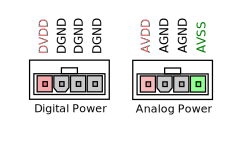
\includegraphics[scale=1.0]{enclosure.back.power.svg}
\caption{The analog and digital power ports. DVDD=+5V, AVDD=+5V, AVSS=-5V. }
\label{power}
\end{figure}
